\externaldocument{main.tex}
Naturally, in a rapidly evolving environment which software engineering and even more so 
web development is, developers have multiple approaches to solving the same issue, which 
in this case would be the development of a web application.
Having outlined why web applications have experienced such a rise in popularity and how
Electron presents a novel concept of overcoming web application's inherent shortcomings, 
it is still of interest to examine other ways of web application development.
Such a different solution is presented by the concept of server-side web development.
In contrast to other architectural approaches (including that of Electron) content 
gets rendered on the server and then delivered to the client. 
Taking frameworks such as Angular as a contrasting example, where the UI gets rendered in 
the browser one can see the stark difference in the way these two approaches differ. \paragraph{}
The following figure presents a way of how a server side flow operates.
\begin{figure}[ht]
    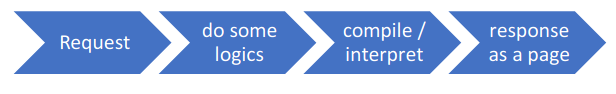
\includegraphics[width=\textwidth]{server-side-flow}
    \caption{Representation of server side flow. \parencite{taufan2020}}
    \label{fig:server-side-flow}
\end{figure}
Naturally a lot of frameworks and tools are available for developers to develop server side
web applications.
One of these tools is Vaadin, a framework for the Java programming language for web development. \parencite{vaadinDocs}
Of course this means Vaadin uses a different approach to web development than Electron 
but the ultimate goal is the same: A web application.
The resulting question is: What advantages and shortcomings does Electron present over other web
development approaches such as server side development?
More specifically in the context of web development multiple question can be asked.
How does performance differ between the two cases? 
Which significant shortcoming and advantages exist for developers?
Where can the advantages of each be best leveraged in a commercial environment? \paragraph{}
As limited previous research exists on this issue a case study following the guidelines 
set by \textcite{caseStudy} will be conducted with the aim of answering the above questions. 
For the case study two cases will be examined: 
One of those being an Electron application and the other a web application 
developed with Vaadin. 
As these cases have to be comparable an implementation of an application with the same functionality 
will be created using both technologies and subsequently compared.
To come to a reliable conclusion data will be collected.
For answering the question of performance, relevant metrics such as measuring time taken for fetching or 
persisting data will be taken. 
This data will then be analised and if applicable any relevant findings presented.
In order to come to reliable answers to the other posed questions observations during development 
will be made.
These observations have to be replicable and must be independent of environment specific variables.